\documentclass[journal,5pt,twocolumn]{IEEEtran}
%
\makeatletter
\makeatother
\usepackage{setspace}
\usepackage{gensymb}
\usepackage{xcolor}
\usepackage{caption}
%\usepackage{stackengine}
%\usepackage{subcaption}
%\doublespacing
\singlespacing



\usepackage{graphicx}
\graphicspath{ {./images}  }
%\usepackage{amssymb}
%\usepackage{relsize}
\usepackage[cmex10]{amsmath}
\usepackage{mathtools}
%\usepackage{amsthm}
\interdisplaylinepenalty=2500
%\savesymbol{iint}
%\usepackage{txfonts}
%\restoresymbol{TXF}{iint}
\usepackage{wasysym}
\usepackage{amsthm}
\usepackage{mathrsfs}
\usepackage{txfonts}
\usepackage{stfloats}
\usepackage{cite}
\usepackage{cases}
\usepackage{mathtools}
\usepackage{subfig}
\usepackage{enumerate}	
\usepackage{enumitem}
\usepackage{amsmath}
%\usepackage{xtab}
\usepackage{longtable}
\usepackage{multirow}
%\usepackage{algorithm}
%\usepackage{algpseudocode}
\usepackage{enumitem}
\usepackage{mathtools}
%\usepackage{iithtlc}
\usepackage{tikz}
\usetikzlibrary{shapes,arrows}
%\usetikzlibrary{arrows.meta,calc,positioning}
%\usepackage[framemethod=tikz]{mdframed}
\usepackage{listings}
    \usepackage[latin1]{inputenc}                                 %%
    \usepackage{color}                                            %%
    \usepackage{array}                                            %%
    \usepackage{longtable}                                        %%
    \usepackage{calc}                                             %%
    \usepackage{multirow}                                         %%
    \usepackage{hhline}                                           %%
    \usepackage{ifthen}                                           %%
  %optionally (for landscape tables embedded in another document): %%
    \usepackage{lscape}     


%\usepackage{stmaryrd}


%\usepackage{wasysym}
%\newcounter{MYtempeqncnt}
\DeclareMathOperator*{\Res}{Res}
%\renewcommand{\baselinestretch}{4}
%\setcounter{secnumdepth}{4}
\renewcommand\thesection{\arabic{section}}
\renewcommand\thesubsection{\thesection.\arabic{subsection}}
\renewcommand\thesubsubsection{\thesubsection.\arabic{subsubsection}}
%\renewcommand\thesubsubsubsection{\thesubsubsection.\arabic{subsubsubsection}}

%\renewcommand\thesectiondis{\arabic{section}}
%\renewcommand\thesubsectiondis{\thesectiondis.\arabic{subsection}}
%\renewcommand\thesubsubsectiondis{\thesubsectiondis.\arabic{subsubsection}}
%\renewcommand\thesubsubsubsectiondis{\thesubsubsectiondis.\arabic{subsubsubsection}}
% correct bad hyphenation here
\hyphenation{Future Wireless communications}

%\lstset{
%language=C,
%frame=single, 
%breaklines=true
%}

%\lstset{
	%%basicstyle=\small\ttfamily\bfseries,
	%%numberstyle=\small\ttfamily,
	%language=Octave,
	%backgroundcolor=\color{white},
	%%frame=single,
	%%keywordstyle=\bfseries,
	%%breaklines=true,
	%%showstringspaces=false,
	%%xleftmargin=-10mm,
	%%aboveskip=-1mm,
	%%belowskip=0mm
%}

%\surroundwithmdframed[width=\columnwidth]{lstlisting}
\def\inputGnumericTable{}                                 %%

\lstset{
%language=python,
frame=single, 
breaklines=true,
columns=fullflexible
}

 

\begin{document}
%
\tikzstyle{block} = [rectangle, draw,
text width=7em, text centered, minimum height=4em]
\tikzstyle{sum} = [draw, circle, node distance=3cm]
\tikzstyle{input} = [coordinate]
\tikzstyle{output} = [coordinate]
\tikzstyle{pinstyle} = [pin edge={to-,thin,black}]
\tikzstyle{line} = [draw, -latex']
\theoremstyle{definition}
\newtheorem{theorem}{Theorem}[section]
\newtheorem{problem}{Problem}
\newtheorem{proposition}{Proposition}[section]
\newtheorem{lemma}{Lemma}[section]
\newtheorem{corollary}[theorem]{Corollary}
\newtheorem{example}{Example}[section]
\newtheorem{definition}{Definition}[section]
%\newtheorem{algorithm}{Algorithm}[section]
%\newtheorem{cor}{Corollary}
\newcommand{\BEQA}{\begin{eqnarray}}
\newcommand{\EEQA}{\end{eqnarray}}
\newcommand{\define}{\stackrel{\triangle}{=}}

\bibliographystyle{IEEEtran}
%\bibliographystyle{ieeetr}

\providecommand{\nCr}[2]{\,^{#1}C_{#2}} % nCr
\providecommand{\nPr}[2]{\,^{#1}P_{#2}} % nPr
\providecommand{\mbf}{\mathbf}
\providecommand{\pr}[1]{\ensuremath{\Pr\left(#1\right)}}
\providecommand{\qfunc}[1]{\ensuremath{Q\left(#1\right)}}
\providecommand{\sbrak}[1]{\ensuremath{{}\left[#1\right]}}
\providecommand{\lsbrak}[1]{\ensuremath{{}\left[#1\right.}}
\providecommand{\rsbrak}[1]{\ensuremath{{}\left.#1\right]}}
\providecommand{\brak}[1]{\ensuremath{\left(#1\right)}}
\providecommand{\lbrak}[1]{\ensuremath{\left(#1\right.}}
\providecommand{\rbrak}[1]{\ensuremath{\left.#1\right)}}
\providecommand{\cbrak}[1]{\ensuremath{\left\{#1\right\}}}
\providecommand{\lcbrak}[1]{\ensuremath{\left\{#1\right.}}
\providecommand{\rcbrak}[1]{\ensuremath{\left.#1\right\}}}
\theoremstyle{remark}
\newtheorem{rem}{Remark}
\newcommand{\sgn}{\mathop{\mathrm{sgn}}}
\providecommand{\abs}[1]{\left\vert#1\right\vert}
\providecommand{\res}[1]{\Res\displaylimits_{#1}} 
\providecommand{\norm}[1]{\lVert#1\rVert}
\providecommand{\mtx}[1]{\mathbf{#1}}
\providecommand{\mean}[1]{E\left[ #1 \right]}
\providecommand{\fourier}{\overset{\mathcal{F}}{ \rightleftharpoons}}
%\providecommand{\hilbert}{\overset{\mathcal{H}}{ \rightleftharpoons}}
\providecommand{\system}{\overset{\mathcal{H}}{ \longleftrightarrow}}
	%\newcommand{\solution}[2]{\textbf{Solution:}{#1}}
\newcommand{\solution}{\noindent \textbf{Solution: }}
\newcommand{\myvec}[1]{\ensuremath{\begin{pmatrix}#1\end{pmatrix}}}
\providecommand{\dec}[2]{\ensuremath{\overset{#1}{\underset{#2}{\gtrless}}}}
\DeclarePairedDelimiter{\ceil}{\lceil}{\rceil}
%\numberwithin{equation}{subsection}
\numberwithin{equation}{section}
%\numberwithin{problem}{subsection}
%\numberwithin{definition}{subsection}
%\makeatletter
%\@addtoreset{figure}{section}
%\makeatother

\let\StandardTheFigure\thefigure
%\renewcommand{\thefigure}{\theproblem.\arabic{figure}}
%\renewcommand{\thefigure}{\thesection}


%\numberwithin{figure}{subsection}

%\numberwithin{equation}{subsection}
%\numberwithin{equation}{section}
%\numberwithin{equation}{problem}
%\numberwithin{problem}{subsection}
%\numberwithin{problem}{section}
%%\numberwithin{definition}{subsection}
%\makeatletter
%\@addtoreset{figure}{problem}
%\makeatother
%\makeatletter
%\@addtoreset{table}{problem}
%\makeatother

\let\StandardTheFigure\thefigure
\let\StandardTheTable\thetable
\let\vec\mathbf
%%\renewcommand{\thefigure}{\theproblem.\arabic{figure}}
%\renewcommand{\thefigure}{\theproblem}

%%\numberwithin{figure}{section}

%%\numberwithin{figure}{subsection}



\def\putbox#1#2#3{\makebox[0in][l]{\makebox[#1][l]{}\raisebox{\baselineskip}[0in][0in]{\raisebox{#2}[0in][0in]{#3}}}}
     \def\rightbox#1{\makebox[0in][r]{#1}}
     \def\centbox#1{\makebox[0in]{#1}}
     \def\topbox#1{\raisebox{-\baselineskip}[0in][0in]{#1}}
     \def\midbox#1{\raisebox{-0.5\baselineskip}[0in][0in]{#1}}




\title{ 
%	\logo{
Implementation of polar codes as per 5G standard
%	}
}



\author{Mannava Venkatasai}% <-this % stops a space



% make the title area
\maketitle
\tableofcontents

\section{\textbf{Introduction}}
\raggedright In recently finalized release-15 5G new radio (NR) access
technology standards by 3rd Generation Partnership Project
(3GPP), two new physical-layer channel coding schemes
of polar and low-density parity-check (LDPC) codes have
been introduced to replace convolutional and Turbo codes.There are three main 5G
usage scenarios of enhanced mobile broadband (eMBB),
ultra-reliable and low latency communications (URLLC),
and massive machine type communications (mMTC).
These scenarios require improved throughput, latency, and
reliability compared with a 4G system.

\section{\textbf{Encoding}}
\subsection{\textbf{Algorithm for polar encoding process}}
\raggedright The polar encoder is the type of encoder which takes K bits as input and gives N bits as output.Where N$\ge$K.As per the 5G standard The Value of N should be 1024. \vspace{5mm} \\
While encoding the message bits in order to achieve efficient communication the K must be small compared to N. \\
The polar encoding process include Two steps.
\begin{enumerate}
\item Adding the frozen bits to the message signal as per the reliability sequence.
\begin{enumerate}
\item As per the 5G standard the size of N must be 1024. So we need the convert the message of length K to N by adding the frozen bits at unreliable positions.
\item As per the Bhattacharya bounds the reliability sequence for the 5G standard in the order from worst to best is given as :
\begin{lstlisting}
https://github.com/Mannava123455/module_2/blob/main/FWC_2_polarencoder/codes/reliability_sequence.dat
\end{lstlisting}
\end{enumerate}
\item Apply polar transform for the manipulated message signal.
\begin{enumerate}
\item The polar transform of the manipulated signal is done by the matrix multiplication of the meanipilated signal with the polar matrix.
\item The basic kernel is given as:
\begin{align}
\vec{G}&=
\begin{pmatrix}
1 & 0 \\
1 & 1 
\end{pmatrix}
\end{align}
\item The Generator matrix for higher values of N is obtained form the kronocker product with same matrix.
\item For example in order to encode the message of length 8.We have to do the kronocker product of the base matrix 3 times.\\
\begin{align}
\vec{G^1}&=
\begin{pmatrix}
1 & 0 \\
1 & 1 
\end{pmatrix}
\end{align}
Perform the kronocker product with same.\\
\begin{align}
\vec{G^2}&=
\begin{pmatrix}
1 & 0 & 0 & 0 \\
1 & 1 & 0 & 0 \\
1 & 0 & 1 & 0 \\
1 & 1 & 1 & 1 
\end{pmatrix}
\end{align}
Again perform the kronocker product with same.\\
\begin{align}
\vec{G^3}&=
\begin{pmatrix}
1 & 0 & 0 & 0 & 0 & 0 & 0 & 0 \\
1 & 1 & 0 & 0 & 0 & 0 & 0 & 0 \\
1 & 0 & 1 & 0 & 0 & 0 & 0 & 0 \\
1 & 1 & 1 & 1 & 0 & 0 & 0 & 0 \\
1 & 0 & 0 & 0 & 1 & 0 & 0 & 0 \\
1 & 1 & 0 & 0 & 1 & 1 & 0 & 0 \\
1 & 0 & 1 & 0 & 1 & 0 & 1 & 0 \\
1 & 1 & 1 & 1 & 1 & 1 & 1 & 1 \\
\end{pmatrix}
\end{align}
If manipulated signal came step 1 is :
\begin{align}
\vec{M}&=
\begin{pmatrix}
1 & 0 & 0 & 0 & 0 & 0 & 0 & 0 
\end{pmatrix}
\end{align}
\item The encoded signal is given as :\\
\begin{align}
\vec{E}&=\vec{M}\vec{G}^3
\end{align}
\end{enumerate}
\end{enumerate}
\subsection{\textbf{Performing BPSK modulation}}
The encoded bits are modulated by using BPSK i.e By changing 0 to 1 and 1 to -1. \\
Now we have a signal that contains -1 and 1.We have an array of size 1024 that has 1 and -1.
\subsection{\textbf{Adding the Noise to the modulated signal}}
In order to analysed the real time communication we have to deal with noise.The modulated signal is being added with noise signal.The noise is analysed by the gaussian signal.\\
The siulation is done by taking different values of SNR in dB.\\
Let us consider the SNR is 2dB.

\begin{align}
SNR&=2 dB \\
EBNo&=10^\frac{SNR}{10} \\
EBNo&=1.5848 \\
Rate&=\frac{K}{N} \\
Rate&=\frac{200}{1024} \\
Rate&=0.1953\\
\sigma&=\frac{1}{\sqrt{2*Rate*EBNo}}
\end{align}
The above $\sigma$ is multiplied with gaussian signal and add it to the BPSK signal.
So that we are having the signal mixed with noise.

\section{\textbf{Decoding}}
\subsection{\textbf{Successive Cancelation Decoding}}
\begin{enumerate}
\item The decoding process includes both Demodulation and Decoding the message signal.\\
The block diagram of Polar encoder is : \\
\begin{figure}[!ht]
\begin{center}
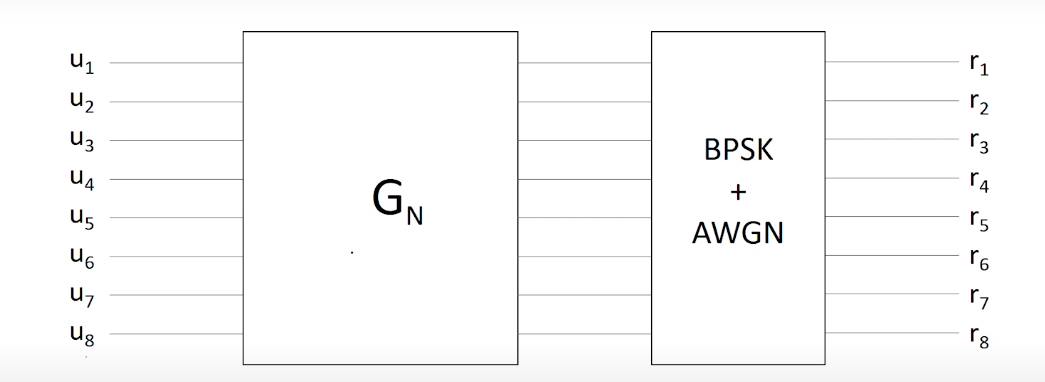
\includegraphics[width=\columnwidth]{/home/mannava/latex/polar.png}
\end{center}
\label{fig : check}
\end{figure}
I the above figure $u_1,u_2......u_8$ are the manipulated message bits and $r_1,r_2,.......,r_8$ are the modulated and encoded bits which will be transmited to the air. \\
The main aim of decoder is to demodulate and decode the transmitted bits.\\
The decoding process is implemented step by step and it is achieved by the Binary search tree algorithm.\\
\begin{figure}[!ht]
\begin{center}
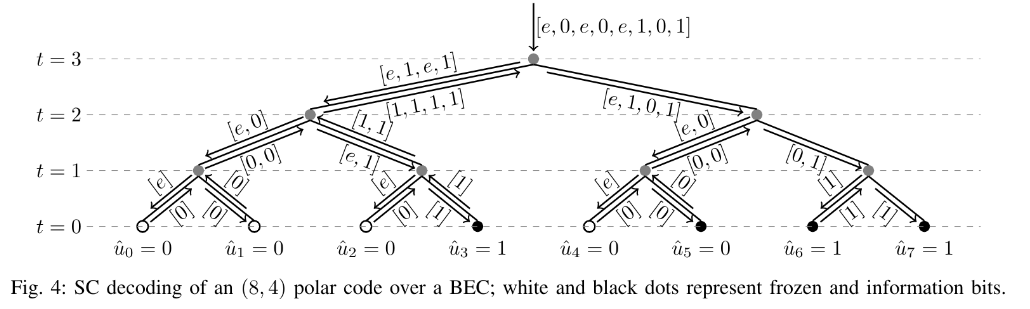
\includegraphics[width=\columnwidth]{/home/mannava/latex/decode.png}
\end{center}
\caption{Check node operation}
\label{fig : check}
\end{figure}
\item The above decoding will be achieved by xoring the bits and by the implementing the to two functions.\\
\begin{enumerate}
\item Step 1:Minsum
\begin{align}
L(u_1)&=f(r_1,r_2)=sgn(r_1)sgn(r_2)min(\abs{r_1},\abs{r_2}) 
\end{align}
\begin{enumerate}
\item $u_1$=0 \\
if L($u_1$) $\ge$ 0
\item $u_1$=1 \\
if L($u_1$) $\le$ 0
\end{enumerate}
\item Step2:
\begin{align}
g(r_1,r_2,b)&=r_2+(1-2b)r_1
\end{align}
\begin{enumerate}
\item $r_2$+$r_1$\\
if b=0
\item $r_2$-$r_1$\\
if b=1
\end{enumerate}
\end{enumerate}
 \end{enumerate}
 By computing the transmited data with the above Steps we will be recovering the message signal from the transmitted signal.
 \section{\textbf{Implementing the polar encoder in python}}
 The polar encoder is implemented in python by using the above algorithm. \\
 The code is uploaded in the below link for polar encoder.\\
 \begin{lstlisting}
 https://github.com/Mannava123455/module_2/blob/main/FWC_2_polarencoder/codes/polar_python/polarencoder.py
 \end{lstlisting}
Analysis of encoded signal with the addition of noise is shown in the figure for SNR = 2dB. \\
Python code for analysis of BPSK is given as :\\
\begin{lstlisting}
import matplotlib.pyplot as plt
import numpy as np
mean = [0, 0]
cov = [[1, 0], [0, 1]]  # diagonal covariance
A = 2
A1=10**(0.1*A);
simlen = int(1024)
n12 = np.random.multivariate_normal(mean, cov, simlen).T
values = [-1, 1]
probabilities = [0.4, 0.6]
X=np.random.choice(values, simlen, p=probabilities)
y_var = A*X + n12
y1=[]
y2=[]
for i in range(0,len(y_var)):
    if (y_var[i]>0):
        y1.append(y_var[i])

for i in range(0,len(y_var)):
    if (y_var[i]<0):
        y2.append(y_var[i])
print(len(y1))
x=np.linspace(-10,10,len(y1))
x1=np.linspace(-10,10,len(y2))
plt.scatter(x,y1,color=['red'])
plt.scatter(x1,y2,color=['green'])
plt.axhline(y = 0, color = 'r', linestyle = '-')
plt.xlabel("$x$")
plt.ylabel("$y$")
plt.legend(["s1","s0"])
plt.savefig('/home/mannava/latex/snr.pdf')
plt.show()
\end{lstlisting}
\begin{figure}[!ht]
\begin{center}
\includegraphics[width=\columnwidth]{/home/mannava/latex/snr.pdf}
\end{center}
\label{fig : check}
\end{figure}

\section{\textbf{Implementing the polar decoder in python}}
\begin{enumerate}
\item The python code for polar decoder is given in the link.\vspace{5mm} 
\begin{lstlisting}
https://github.com/Mannava123455/module_2/blob/main/FWC_2_polarencoder/codes/polar_python/polar_encoder_and_decoder.py
\end{lstlisting}
\item The python code for polar encoder and decoder which is implemented in noisy channel is given in followed link.
\begin{lstlisting}
https://github.com/Mannava123455/module_2/blob/main/FWC_2_polarencoder/codes/polar_python/polarencoder_in_noisychannel.py
\end{lstlisting}
\item Bit error rate analysis \\
BER is given as :\\
\begin{align}
BER = \frac{e}{K}
\end{align}
Where K is no bits transmitted and e is No of errors in recovered signal.
The BER graph is plotted for 10 values of SNR for transmission of 1000 bits :
\begin{figure}[!ht]
\begin{center}
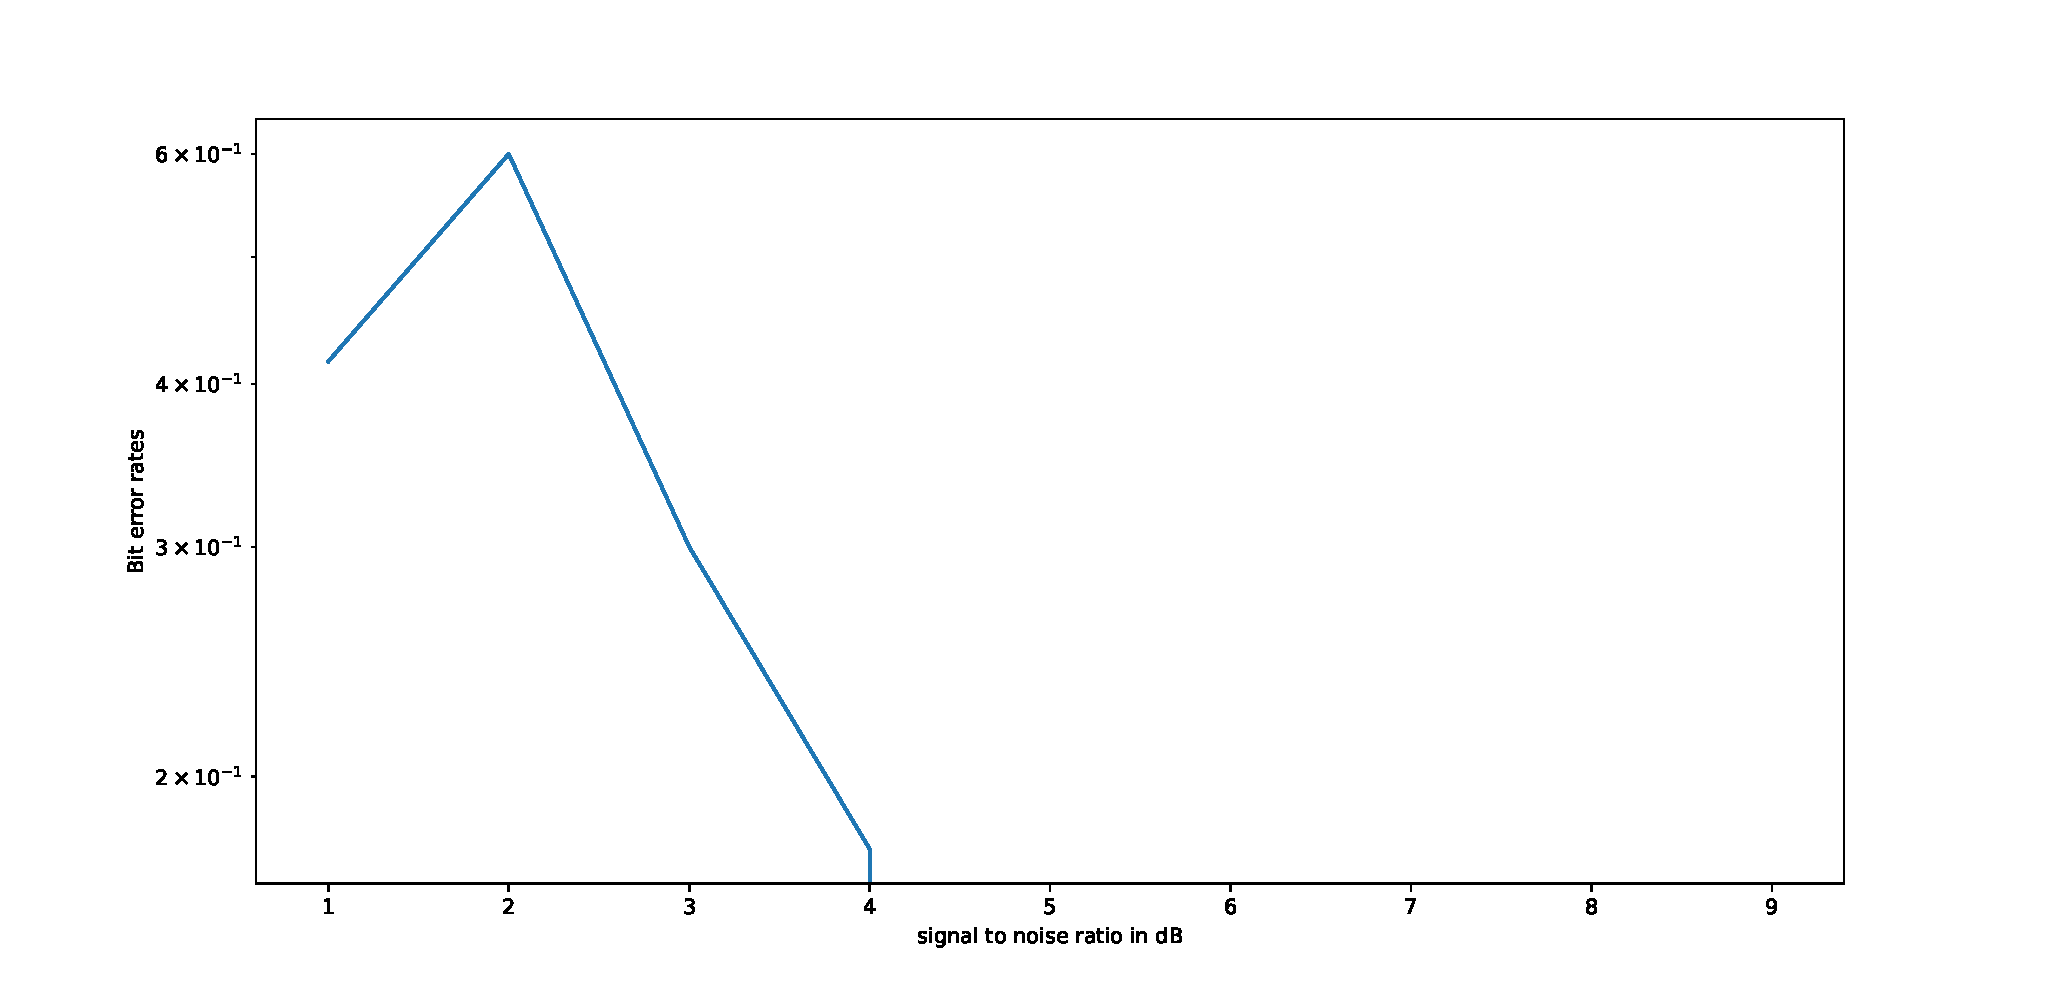
\includegraphics[width=\columnwidth]{/home/mannava/latex/snr1.pdf}
\end{center}
\label{fig : check}
\end{figure}
\end{enumerate}
\section{\textbf{Implementing the polar encoder in C language}}
The polar encoder is implemented in C by using the above algorithm. \\
 The code is uploaded in the below link for polar encoder.\\
 \begin{lstlisting}
 https://github.com/Mannava123455/module_2/blob/main/FWC_2_polarencoder/codes/polar_in_c_language/main.c
 \end{lstlisting}
\section{\textbf{Implementing the polar decoder in C language}}
The polar decoder is implemented in C by using the above algorithm. \\
 The code is uploaded in the below link for polar decoder.\\
 \begin{lstlisting}
https://github.com/Mannava123455/module_2/blob/main/FWC_2_polarencoder/codes/polar_decoder_c/decoder.c
 \end{lstlisting}
\section{\textbf{Implementing the polar encoder in ESP32 in Serial communication manner}}
In this implementation the Arduino board is the transmitter which transmit random bits to Esp32 through UART protocol. \\
There is a FIFO buffer in esp32 of size 200 which continously encode the incoming bits of size 200.\\
The out put is displayed in Serial monitor of ESP32 board.
The project files for implementing polar encoder in esp32 is given in followed link:
\begin{lstlisting}
https://github.com/Mannava123455/module_2/tree/main/FWC_2_polarencoder/codes/polar_encoder_esp32
 \end{lstlisting}



 
 
\end{document}
